\begin{frame}{CT Reconstruction}

\begin{block}{Forward model}
Given by the X-ray transform $\mathcal{R}$:
$$
g = \mathcal{R}f(\theta,s)= \int_{-\infty}^{\infty}\int_{-\infty}^{\infty}f(x,y)\delta(x\cos\theta+y\sin\theta-s)dxdy
$$
where $f\in \mathcal{D}'(\mathbb{R}^2)$.
\end{block}

\pause
\bigskip

\textbf{Ill-posedness:}    
\begin{itemize}
\item Filtered back projection ($R^{-1}$) involves differentiation $\longrightarrow$ increases singularities and noise.
 
\item $R^{-1}$ is unbounded $\longrightarrow$ two far apart images can have very close X-ray transform.
\end{itemize}
\end{frame}


\begin{frame}{Shepp-Logan phantom}
\begin{figure}[!tbp]
  \centering
  \begin{minipage}[b]{0.45\textwidth}
    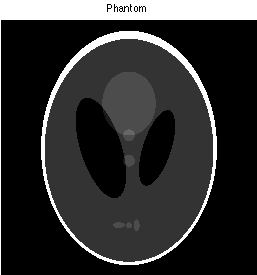
\includegraphics[width=\textwidth]{Images/phantom.png}
  \end{minipage}
  \hfill
  \begin{minipage}[b]{0.45\textwidth}
    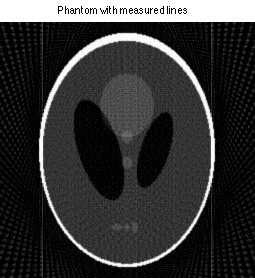
\includegraphics[width=\textwidth]{Images/phantom_measured.png}
  \end{minipage}
\end{figure}
\end{frame}

\begin{frame}{Sinogram}
\begin{figure}[!tbp]
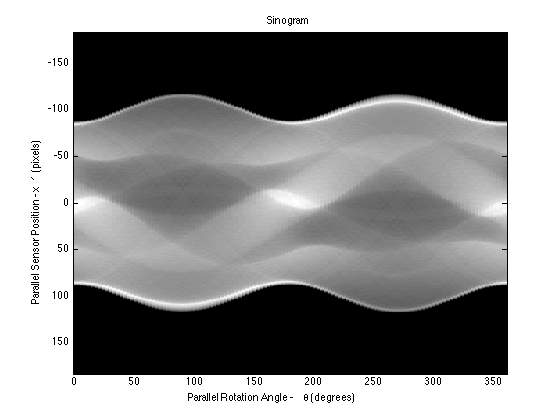
\includegraphics[width=0.9\textwidth]{../sinogram.png}
\end{figure}
\end{frame}

\begin{frame}{Solving inverse problems}
\begin{block}{First approach}
Minimizing the miss-fit against data:
$$
\min_{f} \mathcal{L}(\mathcal{R}(f),g)
$$
e.g. $\mathcal{L}(\mathcal{R}(f),g)=||\mathcal{R}(f)-g||_2^2$.
\end{block}

\textbf{Three classical techniques:}
\begin{itemize}
\item Pseudo-inverse of $\mathcal{T}$ using a mollifier.
\item Iterative regularization, starting with a fixed point iteration scheme for minimizing (iterative hard thresholding), and stop iterates before over-fitting.
\item Variational regularization, by introducing a functional $\mathcal{S}:X\longrightarrow \mathbb{R}$, that encodes a-priori information about $f_{\text{true}}$, e.g.\ sparsity under some dictionary.
$$
\min_{f\in X} [\mathcal{L}(\mathcal{T}f,g)+\lambda \mathcal{S}f] \quad \text{for fixed}\quad \lambda\geq 0
$$
$\lambda$ (regularization parameter) governs the influence of the a priori knowledge, choosing it is a problem.
\end{itemize}
\end{frame}

\begin{frame}{Learning comes into play}

One could ask to learn a pseudo-inverse $\mathcal{T}_{\Theta}(g)\approx f_{\text{true}}$ and learn the parameters $\Theta\in Z$ through a loss functional. 

\pause

\bigskip

Fully learned method are very dependent on the training set, one would like to combine a partially learned iterative method with known information of the problem (e.g.\ wavefront set).

\pause

\bigskip

\begin{itemize}
\item If $\mathcal{T}$ is local (e.g.\ deblurring problem) $\longrightarrow$ convolutional neural network and known pairs $(g,f_{\text{true}})$.
\item If $\mathcal{T}$ is global (e.g.\ Radon transform) $\longrightarrow$ CNN does not work, it becomes unfeasible to work with NN with fully connected layers.
\end{itemize}
\end{frame}

\begin{frame}{Alternative solutions}
\begin{enumerate}
\item Recast to image-to-image problem: perform some initial (non machine-learning) reconstruction (e.g.\ FBP), and then use standard CNN to denoise the initial reconstruction. Upside: it outperforms previous state of the art methods. Donwside: it does not give you more information than using just non-machine learning reconstruction.

\pause 

\item Incorporate enough a-priori information to make the problem tractable and learn the rest (Learned Primal-dual algorithm): First use CNN to update the data (dual step), then apply $\mathcal{T}^*$ and use the result as input to another neural network which updates the reconstruction (primal step), then apply $\mathcal{T}$ and use it as input to a neural network that updates the data, and so on. Upside: it separates the global aspect of the problem into the forward model and its adjoint and only need to learn local aspects. Downside: to train the NN one needs to perform back-propagation through this NN severak times. 
\end{enumerate}
\end{frame}

\begin{frame}{Wavefront set as extra information}
\begin{definition}[N-Wavefront set]
Let $N\in\mathbb{R}$ and $f$ a distribution on $\mathbb{R}^2$. We say $(x,\lambda)\mathbb{R}^2\times \mathbb{R}^2$ is a $N-$regular directed point if there exists a nbd.\ of $U_x$ of $x$, a smooth cutoff function $\Phi$ with $\Phi\equiv 1$ on $U_x$ and a nbd.\ $V_{\lambda}$ of $\lambda$ such that:
$$
(\Phi f)^{\wedge}(\eta)=O((1-|\eta|)^{-N}) \quad \text{for all}\quad \eta=(\eta_1,\eta_2) \quad \text{such that}\quad \frac{\eta_2}{\eta_1}\in V_{\lambda}
$$
The $N-$Wavefront set $WF^N(f)$ is the complement of the $N-$regular directed point. The Wavefront Set $WF(f)$ is defined as 

\begin{equation}
\label{eq:Wavefront-set}
WF(f)=\cup_{N>0}WF^N(f)
\end{equation}
\end{definition}
\textbf{Question?} How can one incorporate extra information from the $N-$Wavefront set of an image by knowing just its Radon Transform.
\end{frame}

\begin{frame}{Answer: Canonical shearlet transform of the sinogram}
\begin{block}{Classical Shearlet Transform}
$$
\langle f,\psi_{a,s,t}\rangle =\int_{\mathbb{R}^2}f(x)\overline{\psi_{a,s,t}(x)}dx
$$
where
$$
\mathcal{SH}(\psi)=\{\psi_{a,s,t}(x):=a^{-3/4}\psi (S_sA_ax-t):(a,s,t)\in \mathbb{R}_+\times\mathbb{R}\times\mathbb{R}^2\}
$$
and

$$
A_a:=
\left(
\begin{matrix}
a^1 & 0 \\
0 & a^{1/2}
\end{matrix}
\right)
\quad
S_s:=
\left(
\begin{matrix}
1 & s \\
0 & 1
\end{matrix}
\right)
$$
\end{block}
\end{frame}

\begin{frame}

\begin{theorem}[Resolution of the Wavefront set by continuous shearlet frames; Grohs, 2011] 
Let $\Psi$ be a Schwartz function with infinitely many vanishing moments in $x_2-$direction. Let $f$ be a tempered distribution and $\mathcal{D}=\mathcal{D}_1\cup\mathcal{D}_2$, where

 $\mathcal{D}_1$ =\{$(t_0,s_0)\in \mathbb{R}^2\times [-1,1]:$ for $(s,t)$ in a nbd.\ $U$ fo $(s_0,t_0)$, $|\mathcal{SH}_{\psi}f(a,s,t)|=O(a^k)$ for all $k\in\mathbb{N}$, with the implied constant uniform over $U$\} and

$\mathcal{D}_2$=\{ $(t_0,s_0)\in\mathbb{R}^2\times (1,\infty]:$ for $(1/s,t)$ in a nbd.\ $U$ of $(s_0,t_0)$, $|\mathcal{SH}_{\psi ^{\nu}}f(a,s,t)|=O(a^k)$ for all $k\in\mathcal{N}$, with the implied constant uniform over $U$\}. Then
$$
WF(f)^c=\mathcal{D}
$$
\end{theorem}

\pause

\begin{theorem}[O. \"Otkem et al., 2008]
Broadly speaking, a point on the $N-$Wavefront set of a distribution corresponds to a point on the $N+1/2-$Wavefront set of its Radon transform, with the corresponding directions.
\end{theorem}
\end{frame}

\begin{frame}{Only thing left: Shearlets on the sinogram}
\begin{itemize}
\item Using results of compactly supported shearlets and shearlets on bounded domains, one can construct a shearlet frame on the space of the sinogram $L^2_{x_1-2\pi}([0,2\pi)\times \mathbb{R})$, given by

$$
\psi_{a,s,t}^{x_1-2\pi}(x_1,x_2):=\sum_{\ell\in\{-1,0,1\}}\psi_{a,s,t}(x_1+2\pi\ell,x_2)
$$
where $\psi_{a,s,t}$ is a shearlet compactly supported on $[0,2\pi)\times \mathbb{R}$, whose corresponding system form a frame for $L^2([0,2\pi)\times \mathbb{R})$.

\pause

\item Then in the learned primal-dual algorithm one can incorporate as extra information the $N-$Wavefront set of the image by pulling back the $N+1/2-$Wavefront set captured by the proposed shearlet frame. This will let us to get a solution with minimum lost of the important features of the images.
\end{itemize}
\end{frame}

\begin{frame}{Thanks!}
\begin{center}
\Large{Questions?}
\end{center}
\end{frame}

